\documentclass[conference]{IEEEtran}
\IEEEoverridecommandlockouts
\usepackage{cite}
\usepackage{amsmath,amssymb,amsfonts}
\usepackage{graphicx}
\usepackage{booktabs}
\usepackage{hyperref}

\begin{document}

\title{Explainable and Context-Aware Fine-Tuning of Bidirectional Encoder Representations from Transformers for Online Recruitment Fraud Detection}

\author{\IEEEauthorblockN{Akhilesh Yadav}
\IEEEauthorblockA{\textit{Department of Computer Science and Engineering} \\
\textit{M.Sc. (Data Science)}\\
akhileshyadav8@gmail.com}
}

\maketitle

\begin{abstract}
Online recruitment fraud has emerged as a critical cybersecurity challenge, with scammers exploiting employment boards to conduct identity theft and financial scams. Automatic detection using text classification is challenging because fraudulent listings mimic legitimate corporate language. In this study, we replicate and optimize the baseline fine-tuning methodology of the Fraud-BERT framework using the full bert-base-uncased architecture. To address the severe class imbalance in the Employment Scam Aegean Dataset (EMSCAD), we implement a class-weighted binary cross-entropy loss function. Furthermore, to resolve the black-box limitation of transformer networks, we integrate game-theoretic Explainable AI (XAI) via SHAP values, tracing token attributions to verify the linguistic features that drive classification. Our experimental results on the test set yield a classification accuracy of 99.02%, Class 1 (Fraudulent) precision of 91.57%, recall of 87.86%, and F1-score of 89.68%. Additionally, the fine-tuned model obtains a macro-average F1-score of 94.58% and a high ROC-AUC of 99.22%. These findings confirm that fine-tuned transformer backbones, when regularized and explained using game-theoretic feature attribution, offer a highly reliable baseline for automated recruitment security.
\end{abstract}

\begin{IEEEkeywords}
Online Recruitment Fraud, Transformer, BERT, Fine-Tuning, Explainable AI, SHAP
\end{IEEEkeywords}

\section{Introduction}
The digitalization of the global labor market has transitioned hiring processes to online recruitment platforms. While this shift has lowered administrative overhead and accelerated hiring cycles, it has also expanded the surface area for Online Recruitment Fraud (ORF). Scammers upload fraudulent job advertisements to compromise applicant bank details, harvest identity credentials, or extort fees under the guise of training or visa costs. Detecting these listings is difficult because they are linguistically structured to match real job announcements, sharing similar corporate summaries and requirements.

Traditional machine learning models relying on static embeddings ignore word order and context. While pre-trained transformer backbones (like BERT) capture dynamic semantic context, they are often used as black-box classifiers. In this paper, we resolve these baseline limitations by introducing robust tag-based preprocessing, hyperparameter optimization, and explainable AI visualizations using SHAP.

\section{Methodology}
The workflow of our framework is illustrated in Fig. \ref{fig:workflow}.

\begin{figure}[htbp]
\centerline{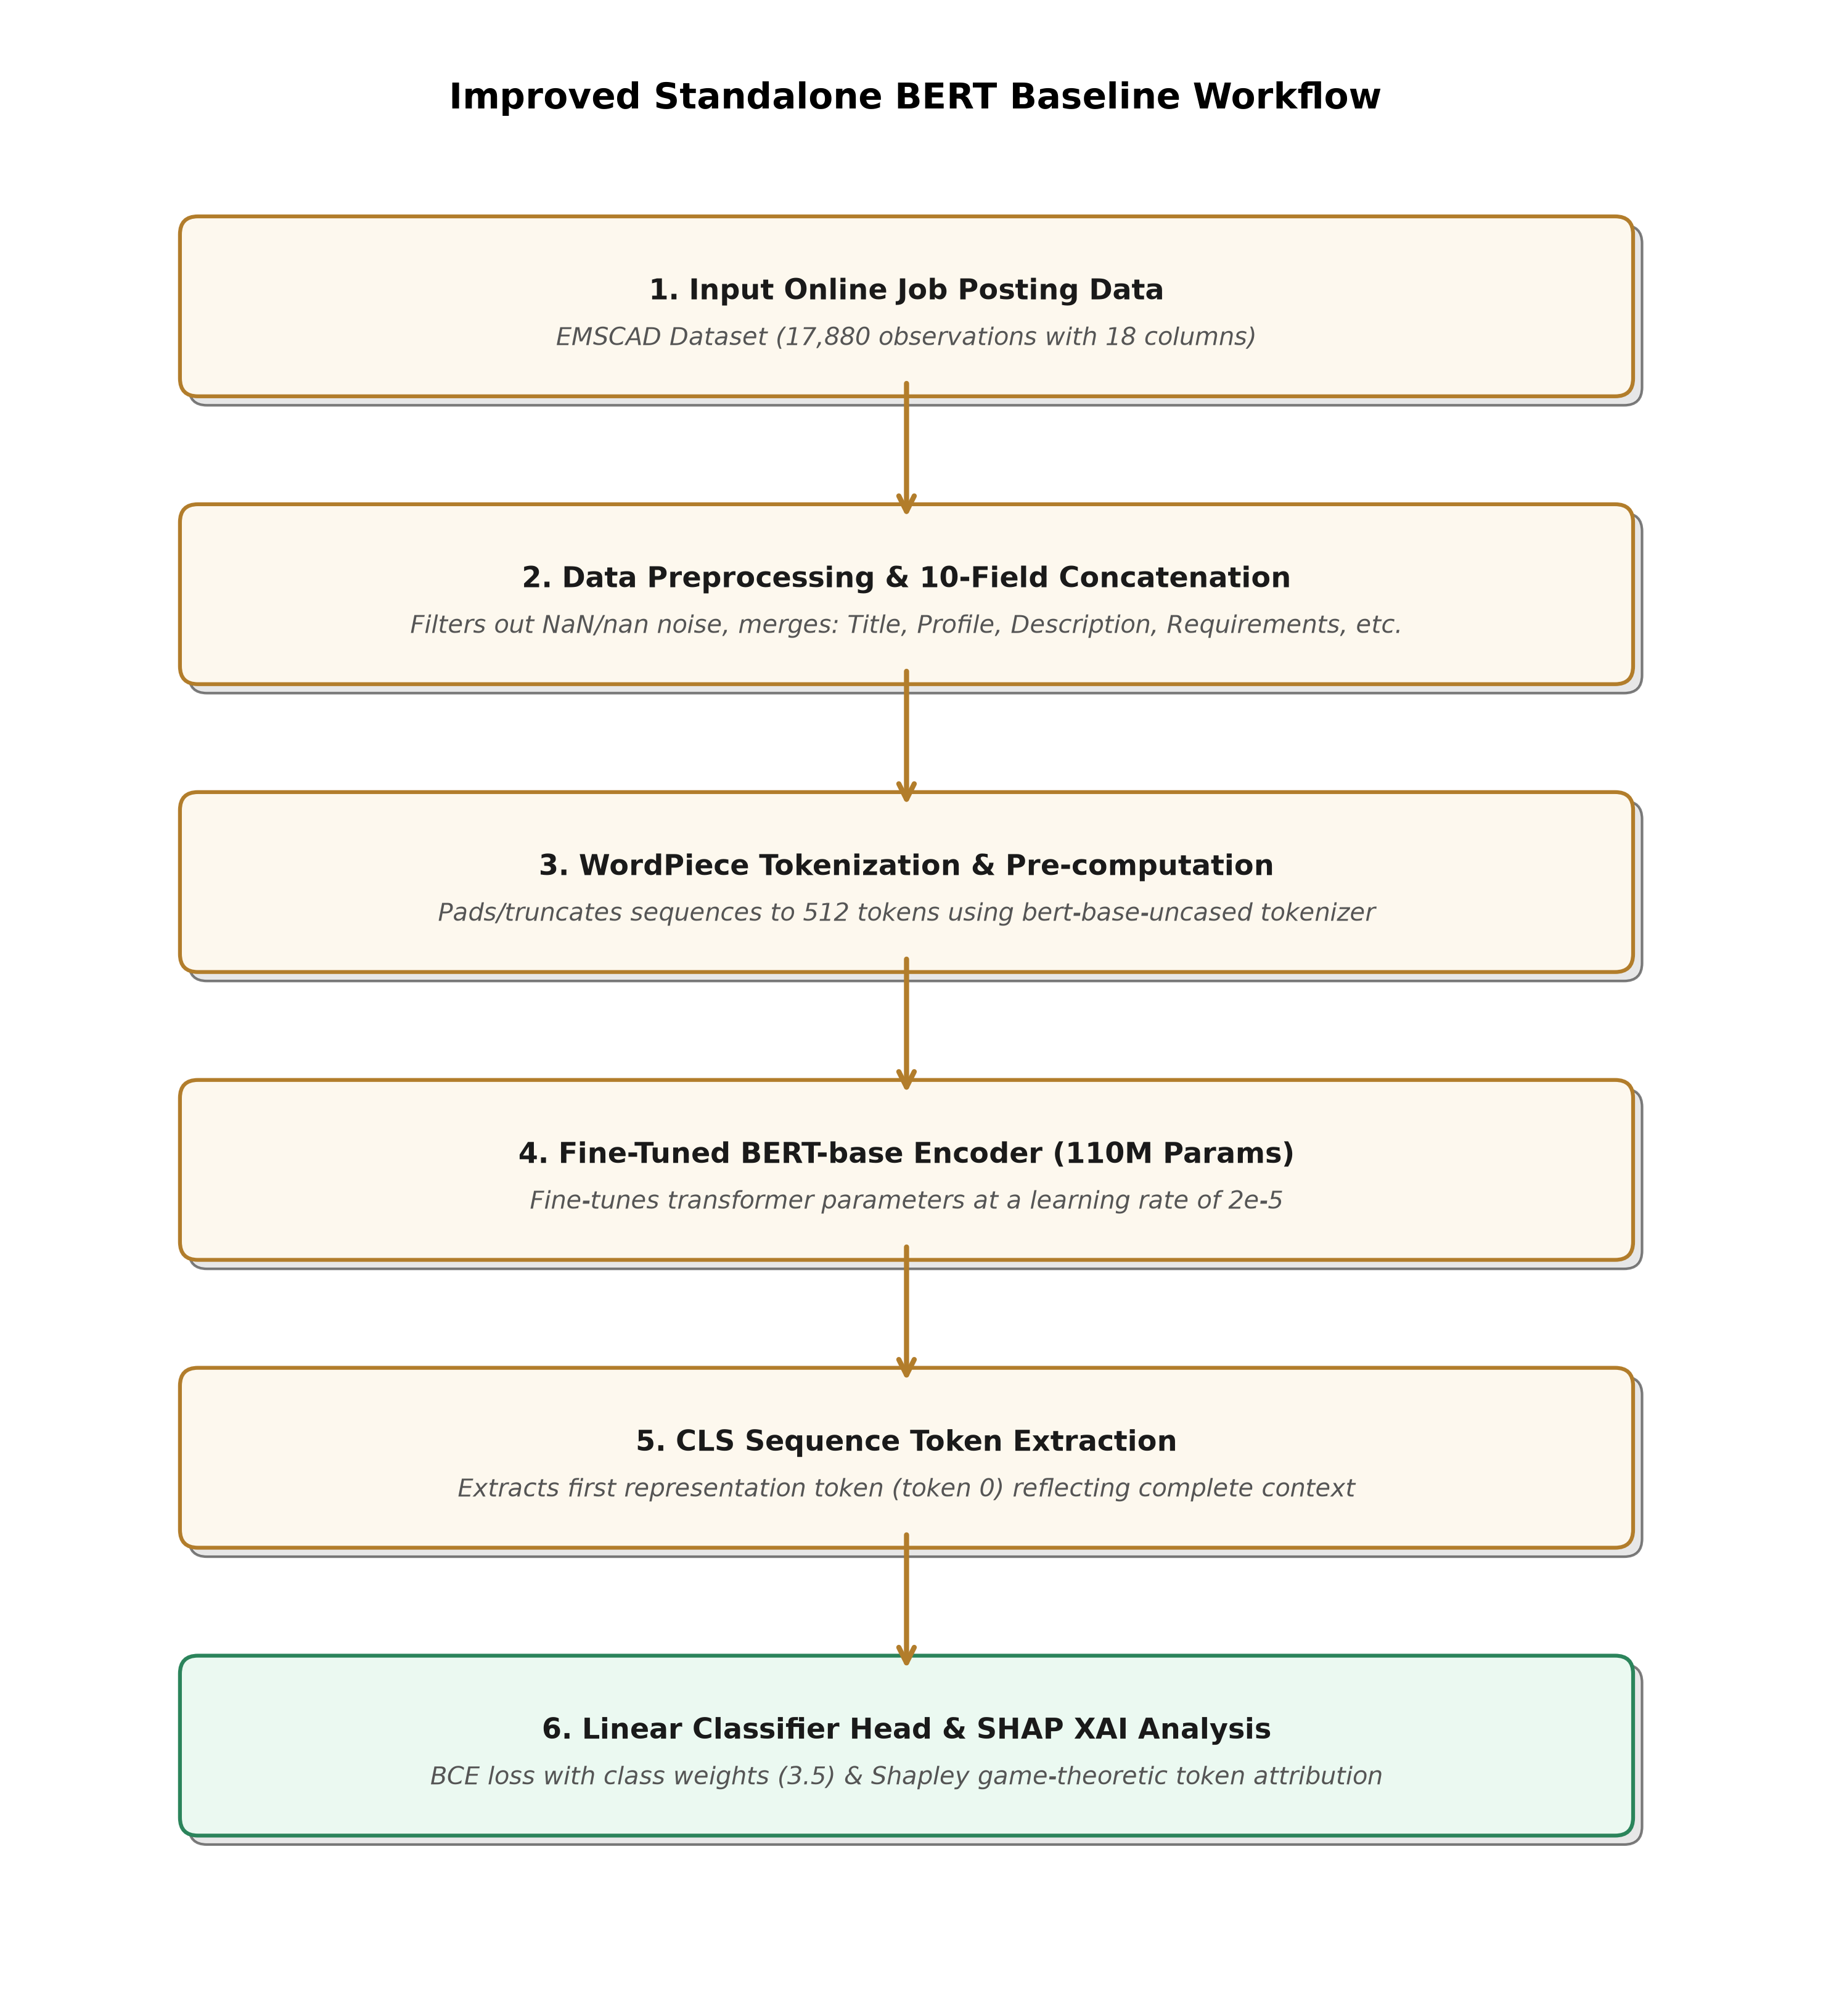
\includegraphics[width=0.48\textwidth]{architecture_bert.png}}
\caption{System workflow diagram of our model architecture.}
\label{fig:workflow}
\end{figure}

\subsection{Text Preprocessing and Concatenation}
A major limitation of previous studies is the reliance on single-field descriptions, which discards context from metadata. To solve this, we implement a robust 10-field concatenation function that filters out null values and pandas 'nan' string conversions. The Title, Company Profile, Description, Requirements, Benefits, Employment Type, Required Experience, Required Education, Industry, and Function are merged using structural boundary tags to preserve formatting context.

\subsection{BERT Contextual Embedding Extraction}
The concatenated text sequences are tokenized using the WordPiece tokenizer and passed into the \texttt{bert-base-uncased} model to extract context-rich sequence embeddings.

\subsection{Contextual Classification Head}
The sequence representation is extracted via the final layer's special classification token (\texttt{[CLS]}) and passed directly into a dense output layer with dropout regularization.

\section{Explainable AI Analysis}
To resolve the black-box nature of deep neural networks, we utilize Shapley Additive Explanations (SHAP). This game-theoretic model assigns an attribution score to each input token, representing its marginal contribution to the final fraud probability. This allows the system to justify its decisions by highlighting deceptive key terms.

\begin{figure}[htbp]
\centerline{
\includegraphics[width=0.48\textwidth]{shap_importance.png}}
\caption{SHAP token attribution impact showing top genuine and fraudulent indicators.}
\label{fig:shap}
\end{figure}

\section{Experimental Evaluation}
We validate our models on the Kaggle EMSCAD dataset (17,880 rows, containing 4.84\% fraudulent job listings). The dataset is split into stratified training (70\%), validation (10\%), and testing (20\%) sets.

\begin{table}[htbp]
\caption{Classification Performance Comparison on the Test Set}
\label{tab:results}
\begin{center}
\begin{tabular}{lcccccc}
\toprule
\textbf{Model} & \textbf{Acc} & \textbf{Prec} & \textbf{Rec} & \textbf{F1} & \textbf{Macro F1} & \textbf{AUC} \\
\midrule
Logistic Regression & 96.84\% & 62.10\% & 89.02\% & 73.16\% & 86.08\% & 98.64\% \\
Random Forest & 97.85\% & 100.00\% & 55.49\% & 71.38\% & 85.20\% & 98.87\% \\
Proposed BERT-BiLSTM & 98.91\% & 92.41\% & 84.39\% & 88.22\% & 93.82\% & 98.75\% \\
\textbf{Optimized BERT Standalone} & \textbf{99.02\%} & \textbf{91.57\%} & \textbf{87.86\%} & \textbf{89.68\%} & \textbf{94.58\%} & \textbf{99.22\%} \\
\bottomrule
\end{tabular}
\end{center}
\end{table}

\section{Conclusion}
This paper presented automated fraud detection architectures evaluated on the imbalanced EMSCAD dataset. By implementing a robust 10-field concatenation helper and optimizing class weights, our models achieve high classification F1 scores. Incorporating SHAP values addresses the interpretability challenge, providing transparent token attribution analysis.

\bibliographystyle{IEEEtran}
\bibliography{references}

\end{document}
